\section{Các giao thức}
\subsection{AMQP}
\subsubsection{Định nghĩa}
Advanced Message Queuing Protocol (AMQP) là một chuẩn mở định nghĩa một giao thức chung cho các hệ thống trao đổi thông điệp.
\subsubsection{Các khái niệm trong AMQP}
\begin{itemize}
	\item Broker: là một ứng dụng trung gian có thể nhận thông điệp được gửi đến từ bên gửi và phân phối cho bên nhận hoặc các ứng dụng trung gian khác(brokers).
	\item Virtual host: Đây là một bộ phận ảo trong một ứng dụng trung gian (broker) cho phép sự phân biệt của bên gửi, bên nhận và tất cả các thành phần AMQP mà chúng phụ thuộc.
	\item Connection: Đây là một kết nối mạng vật lý (TCP) giữa một
producer/consumer và broker.
	\item Channel: Đây là một kết nối logic giữa một producer/consumer và một broker. Nhiều kênh có thể được thành lập trong một kết nối duy nhất. Kênh cho phép cô lập của sự tương tác giữa một consumer cụ thể và broker để không cản trở nhau. Điều này xảy ra mà không có mở các kết nối TCP cá nhân tốn kém. Một kênh có thể đóng khi một có lỗi giao thức xảy ra.
	\item Exchange: Đây là đích cho tất cả các thông điệp được gửi đến và là thực thể chịu trách nhiệm áp dụng các quy tắc định tuyến đảm bảo cho các thông điệp gửi đến đúng điểm đến. Quy tắc định tuyến gồm: direct (point-to-point), topic (publish-subscribe) và fanout (multicast).
	\item Queue: Đây là điểm đến cuối cùng của thông điệp, thông điệp trong queue sẵn sàng được phân phối cho các consumers. Một tin nhắn có thể được sao chép và đưa đến nhiều queue nếu như quy tắc định tuyến của exchange quy định.
	\item Binding: là một kết nối ảo giữa một exchange và một queue cho phép thông điệp từ exchange sang queue để phân phối cho các consumers. Một routing key có thể liên kết với một ràng buộc trong mối quan hệ các quy tắc trao đổi định tuyến.
\end{itemize}
\begin{figure}[h]
    \centering
    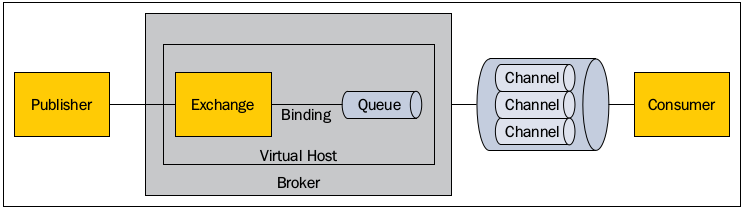
\includegraphics[width=1\textwidth]{amqp-specification}
    \caption{Tổng quan về các khái niệm trong AMQP}
    \label{fig:mesh1}
\end{figure}

\subsection{STOMP}
\subsubsection{Định nghĩa}
Simple Text-Orientated Messaging Protocol là một giao thức tương thích đơn giản được thiết kế cho thông điệp không đồng bộ giữa clients và các máy chủ trung gian. Nó định nghĩa văn bản dựa trên wire-format cho các thông điệp giữa client - server.

\section{Một số khái niệm}
\subsection{Consumers và Producers}